\documentclass[10pt,twocolumn]{article}
\usepackage[a4paper,top=0.55in,bottom=0.55in,left=0.55in,right=0.55in,columnsep=0.22in]{geometry}
\usepackage{amsmath,amssymb,amsfonts}
\usepackage{graphicx}
\usepackage{booktabs}
\usepackage{array}
\usepackage{enumitem}
\usepackage[font={small},labelfont={bf,color=primary},skip=3.0pt]{caption}
\usepackage{titlesec}
\usepackage[table]{xcolor}
\usepackage{microtype}
\usepackage{newtxtext,newtxmath}
\usepackage[colorlinks=true,linkcolor=primary,citecolor=primary,urlcolor=secondary]{hyperref}

\graphicspath{
  {figures/}
  {../results/runs/v4/figures/}
  {../experiments/06_pest_loss_sweep/}
  {../experiments/12_layout_plus_forecast/}
  {../experiments/}
  {FarmRL/results/runs/v4/figures/}
  {FarmRL/experiments/06_pest_loss_sweep/}
  {FarmRL/experiments/12_layout_plus_forecast/}
}

% =========================================================================
% Color Palette & Accents
% =========================================================================
\definecolor{primary}{RGB}{16, 44, 87}         % Academic Deep Navy
\definecolor{secondary}{RGB}{28, 80, 140}      % Cobalt Accent
\definecolor{tableheader}{RGB}{236, 242, 248}  % Header Tint
\definecolor{rowtint}{RGB}{248, 250, 253}      % Alternating Row
\definecolor{cardbg}{RGB}{244, 248, 252}       % Highlight Row Tint
\definecolor{accentred}{RGB}{165, 30, 30}      % Subdued Red Accent

% Section Headings
\titleformat{\section}
  {\normalfont\normalsize\bfseries\color{primary}}
  {\thesection.}{0.4em}{}

\titleformat{\subsection}
  {\normalfont\small\bfseries\color{secondary}}
  {\thesubsection}{0.35em}{}

\titlespacing*{\section}{0pt}{4.5pt plus 1.0pt minus 0.8pt}{1.8pt plus 0.5pt}
\titlespacing*{\subsection}{0pt}{3.5pt plus 0.8pt minus 0.5pt}{1.5pt plus 0.4pt}

% Typography & Spacing
\setlength{\parindent}{0pt}
\setlength{\parskip}{2.2pt plus 0.4pt minus 0.4pt}
\setlength{\textfloatsep}{4.0pt plus 1.0pt minus 1.0pt}
\setlength{\floatsep}{3.5pt plus 1.0pt minus 0.8pt}
\setlength{\intextsep}{3.5pt plus 1.0pt minus 0.8pt}
\setlength{\abovedisplayskip}{2.5pt plus 0.6pt minus 0.6pt}
\setlength{\belowdisplayskip}{2.5pt plus 0.6pt minus 0.6pt}

% High-capacity float controls for two-column balance
\renewcommand{\topfraction}{0.95}
\renewcommand{\bottomfraction}{0.95}
\renewcommand{\textfraction}{0.05}
\renewcommand{\floatpagefraction}{0.85}
\setcounter{topnumber}{3}
\setcounter{bottomnumber}{2}
\setcounter{totalnumber}{5}

% Bullet List Styling
\setlist[itemize]{leftmargin=1.15em,itemsep=0.8pt,topsep=0.8pt,parsep=0pt}

\definecolor{cropgreen}{RGB}{20, 88, 40}       % Dark Agricultural Crop Foliage Green
\definecolor{dirtbrown}{RGB}{138, 86, 42}      % Medium Loamy Soil / Dirt Brown

\newlength{\croptitlewidth}
\begin{document}
\fontsize{9.3pt}{11.3pt}\selectfont

% =========================================================================
% TITLE BLOCK
% =========================================================================
\twocolumn[{%
\begin{@twocolumnfalse}
\settowidth{\croptitlewidth}{\fontsize{13.6pt}{16.2pt}\selectfont \textbf{FarmRL: Reinforcement Learning for Crop Input Management and Market Timing}}
\begin{center}
    {\fontsize{13.6pt}{16.2pt}\selectfont \textbf{\color{cropgreen}FarmRL: Reinforcement Learning for Crop Input Management and Market Timing}}\\[2.5pt]
    {\color{dirtbrown}\rule{\croptitlewidth}{1.5pt}}\\[4.0pt]
    {\normalsize \textbf{Harshita Vachhani} (B23EE1026) \quad and \quad \textbf{Aurindum Banerjee} (B23CS1006)}\\[2.0pt]
    {\small CSL3090: Artificial Intelligence (Assignment 2) $\;\cdot\;$ Indian Institute of Technology Jodhpur}\\
    {\footnotesize \textbf{GitHub Repository \& Live Dashboard:} \href{https://github.com/Harshita772/FarmRL}{\color{secondary}\texttt{https://github.com/Harshita772/FarmRL}}}
\end{center}
\vspace{-4pt}
\noindent{\color{dirtbrown!75}\hrule height 0.7pt}
\vspace{5.0pt}
\end{@twocolumnfalse}
}]

% =========================================================================
% SECTION 1: PROBLEM CONTEXT
% =========================================================================
\section{Problem Context}
Wheat cultivation across the Indo-Gangetic plains follows a six-month Rabi cycle (November to April). Farmers make recurring fortnightly decisions on nitrogen fertilizer ($N$), irrigation water ($W$), and pesticide sprays ($P$), concluding with a market timing choice at harvest ($M$): selling immediately or storing grain for 1--2 months. Standard government extension calendars prescribe fixed, calendar-driven inputs regardless of transient weather. In northwest India (Punjab and Haryana), this practice has driven severe groundwater depletion from tubewell over-pumping, topsoil waterlogging during unseasonal winter rains, nitrate leaching into aquifers, and accelerating pesticide resistance. Dynamic, state-contingent input management is therefore essential for sustainable crop production.

% =========================================================================
% SECTION 2: BUILDING THE RL ENVIRONMENT FROM REAL DATA
% =========================================================================
\section{Constructing the Environment from Empirical Data}
To prevent artificial simulation artifacts, we built the \textbf{FarmRL} Gymnasium environment by calibrating crop growth, weather sequences, and operating costs directly against published Indian agricultural records.

\textbf{1. Climate Replay (NASA POWER):}
The environment replays 39 historical seasons (1985--2023) of daily weather for Ludhiana (Punjab) and Karnal (Haryana), tracking precipitation $R_t$, min/max temperature, solar radiation, relative humidity, and Penman-Monteith reference evapotranspiration $\text{ET}_{0,t}$. Seasons 1985--2016 (32 seasons) are used for training; 2017--2023 (7 unseen seasons $\times$ 30 stochastic replicates) are held out for generalization testing.

\textbf{2. Yield Response Panel Model (ICRISAT):}
Harvest yield $Y$ (q/ha) is modeled through a panel regression fitted on 1,719 district-year observations across 13 Indian states from the ICRISAT-TCI database (held-out $R^2 = 0.512$ with state fixed effects). The biophysical response integrates a Mitscherlich nitrogen curve with FAO-33 water deficit response, stage-specific aeration hypoxia $\bar{\sigma}^{\text{aer}}_g$ (FAO-66), pest damage ($L_p$), and extreme heat-stress days ($H_{\text{days}}$):
\begin{equation}
\begin{aligned}
Y &= A_{\text{state}}\, y_{\text{scale}} \big(1 - e^{-\alpha_N (N_{\text{eff}} + N_0)}\big) \Big(1 - k_y\Big(1 - \tfrac{\text{ET}^{\text{cum}}_a}{\text{ET}^{\text{cum}}_c}\Big)\Big) \\
&\quad \times \prod_{g=1}^{4}\big(1 - K_{y,g}\bar{\sigma}^{\text{aer}}_g\big) \big(1 - L_p D_{\text{pest}}\big) \big(1 - \alpha_H H_{\text{days}}\big)
\end{aligned}
\end{equation}

\textbf{3. Cost Calibration (CACP):}
Unit costs are calibrated to official CACP (2024--25) wheat price policy tables: nitrogen fertilizer $c_N = 12.9\text{ INR/kg}$, canal and diesel irrigation delivery $c_W = 2.86\text{ INR/mm}$, chemical pesticide $c_P = 1{,}183\text{ INR/dose}$, and fixed non-input labor and machinery expenses $C_{\text{fixed}} = 29{,}450\text{ INR/ha}$. Grain revenue follows the Minimum Support Price ($2{,}425\text{ INR/q}$) adjusted by Agmarknet market price indices.

\textbf{4. Four Biophysical Dynamics:}
\begin{itemize}
    \item \textit{Groundwater Drawdown:} Tubewell pumping cost scales directly with water-table lift ($25\text{ m}$ base lift in 2024, secular decline of $0.5\text{ m/year}$ plus intra-season drawdown), consuming $0.02725\text{ kWh/mm}\cdot\text{ha/m}$.
    \item \textit{Waterlogging \& Leaching:} Root zone holds $150\text{ mm}$ available water. Moisture exceeding $45\text{ mm}$ above field capacity drains at $20\text{ mm/day}$, causing root hypoxia (FAO-66) and leaching up to $50\%$ of active soil mineral nitrogen.
    \item \textit{Pest Resistance:} Pest outbreaks follow humidity shocks; each chemical application degrades subsequent pesticide efficacy by $25\%$.
    \item \textit{Storage Market:} Stored grain incurs monthly warehouse fees ($10\text{ INR/q/mo}$), interest ($0.58\%/\text{mo}$), and physical grain loss ($0.3\%/\text{mo}$) under Ornstein-Uhlenbeck price drift ($+1\%/\text{mo}$, $3\%$ volatility).
\end{itemize}

\textbf{5. MDP Formalization ($T=12$ fortnights):}
\begin{itemize}
    \item \textbf{State Space ($\mathcal{S}$):} Normalized 13-dimensional continuous vector (extended to 14-D when a next-fortnight rain forecast $\hat{R}_t$ is supplied):
    \begin{equation}
    \begin{aligned}
    s_t = \Big[
    &\tfrac{t}{T},\; m_t,\; \tfrac{N^{\text{soil}}_t}{100},\; p_t,\; \tfrac{R^{\text{cum}}_t}{200},\; \tfrac{N^{\text{cum}}_t}{200},\; \tfrac{W^{\text{cum}}_t}{500},\\
    &I^{\text{price}}_s,\; \tfrac{R_{t-1}}{50},\; \tfrac{\text{ET}_{0,t-1}}{100},\; \tfrac{\text{ET}^{\text{cum}}_{a,t}}{\text{ET}^{\text{cum}}_{c,t}},\; \tfrac{c^{\text{pump}}_t}{20},\; e^{\text{spray}}_t
    \Big]^\top
    \end{aligned}
    \end{equation}
    capturing stage $t/T$, root moisture $m_t$, soil nitrogen $N^{\text{soil}}_t$, pest pressure $p_t$, cumulative inputs, weather lags, water satisfaction, pumping cost, and remaining spray efficacy.
    \item \textbf{Action Space ($\mathcal{A}$):} Factored $\text{MultiDiscrete}([3, 3, 3, 3])$ ($|\mathcal{A}|=81$): nitrogen $N_t \in \{0, 20, 40\}\text{ kg/ha}$, irrigation $W_t \in \{0, 37.5, 75\}\text{ mm}$, pesticide $P_t \in \{0, 1, 2\}$, and grain storage $M \in \{0, 1, 2\}\text{ months}$ (masked until harvest step $t=11$).
    \item \textbf{Reward Function ($\mathcal{R}$):} Farm net profit minus environmental externalities, scaled by $S_R = 10{,}000$ ($r_t = R_t / S_R$):
    \begin{equation}
    \begin{aligned}
    R_t &= -\big(c_N N_t + c_W W_t + c_P P_t + C^{\text{pump}}_t(W_t)\big) \\
    &\quad -\big(\lambda_N [N^{\text{soil}}_{t+1} - 80]_+ + \lambda_P P_t\big) + \mathbb{I}_{[t = 11]}\big(\text{Rev}_T - C_{\text{fixed}}\big)
    \end{aligned}
    \end{equation}
    where $\lambda_N = 5\text{ INR/kg}$ penalizes soil nitrogen leaching above safe levels and $\lambda_P = 100\text{ INR/dose}$ penalizes excessive chemical usage.
\end{itemize}

% =========================================================================
% SECTION 3: BASELINE POLICIES & BENCHMARKING
% =========================================================================
\section{Baseline Policies and Fair Benchmarking}
To ensure fair evaluation, we benchmark RL against five non-RL policies:
\begin{itemize}
    \item \textbf{No-Input Baseline:} Natural soil fertility without intervention ($17.1\text{ q/ha}$ yield, $12{,}234\text{ INR/ha}$ profit).
    \item \textbf{Random Policy:} Uniform random actions, setting a sanity floor ($55{,}336\text{ INR/ha}$).
    \item \textbf{Recommended Calendar:} Standard Punjab extension advice (120 kg N across 3 splits, 4 irrigations of 75 mm, 1 spray, harvest sale; $74{,}649\text{ INR/ha}$).
    \item \textbf{Untuned Threshold Rule:} Standard textbook moisture and pest thresholds ($62{,}780\text{ INR/ha}$).
    \item \textbf{Tuned Threshold Rule:} Cutoffs optimized via coordinate grid search exclusively on the 32 training seasons (apply 40 kg N if soil N $<100\text{ kg/ha}$; irrigate 75 mm if moisture $<10\%$ and 37.5 mm if $<60\%$; zero spray under calibrated pest loss). Achieves \textbf{$87{,}232\text{ INR/ha}$} on held-out seasons. A retuned calendar achieves $81{,}072\text{ INR/ha}$.
    \item \textbf{Hindsight Foresight Oracle:} Theoretical performance ceiling via cross-entropy plan search endowed with clairvoyance of future daily weather and harvest prices (\textbf{$89{,}654\text{ INR/ha}$}).
\end{itemize}

% =========================================================================
% SECTION 4: EXPERIMENTS, BEST MODEL & LESSONS LEARNED
% =========================================================================


\begin{table}[t]
\centering
\caption{Held-out test performance across 7 unseen Punjab seasons (2017--2023; mean $\pm$ std over 5 seeds, 30 replicates/season).}
\label{tab:results}
\resizebox{\columnwidth}{!}{%
\setlength{\tabcolsep}{3.0pt}
\renewcommand{\arraystretch}{0.96}
\begin{tabular}{lrrrrr}
\toprule
\rowcolor{tableheader}
\textbf{Policy / Configuration} & \textbf{Profit (INR/ha)} & \textbf{\% Orac.} & \textbf{Yield} & \textbf{Irrig.} & \textbf{Sprays} \\
\midrule
Hindsight Oracle (ceiling) & $89{,}654$ & $100.0\%$ & $51.2$ & $225$ & $0.00$ \\
Tuned Threshold Rule & $87{,}232$ & $97.3\%$ & $50.6$ & $241$ & $0.00$ \\
\rowcolor{rowtint}
\textbf{PPO (base \texttt{v4}, 5 seeds)} & $\mathbf{86{,}584 \pm 153}$ & $\mathbf{96.6\%}$ & $\mathbf{50.3}$ & $\mathbf{220}$ & $\mathbf{0.00}$ \\
\textbf{GRPO (critic-free, $G=16$)} & $\mathbf{86{,}223 \pm 680}$ & $\mathbf{96.2\%}$ & $\mathbf{50.1}$ & $\mathbf{232}$ & $\mathbf{0.01}$ \\
CEM (rule parameter search) & $84{,}178 \pm 192$ & $93.9\%$ & $50.4$ & $238$ & $3.46$ \\
Branching Dueling DQN & $83{,}617 \pm 1{,}741$ & $93.3\%$ & $49.5$ & $221$ & $0.83$ \\
Tuned Calendar Rule & $81{,}072$ & $90.4\%$ & $48.4$ & $300$ & $0.00$ \\
Recommended Calendar (Govt) & $74{,}649$ & $83.3\%$ & $45.8$ & $300$ & $1.00$ \\
Untuned Threshold Rule & $62{,}780$ & $70.0\%$ & $45.9$ & $236$ & $11.80$ \\
Random Policy & $55{,}336$ & $61.7\%$ & $44.9$ & $458$ & $11.80$ \\
No-Input Baseline & $12{,}234$ & $13.6\%$ & $17.1$ & $0$ & $0.00$ \\
\bottomrule
\end{tabular}%
}
\end{table}

\begin{figure}[t]
    \centering
    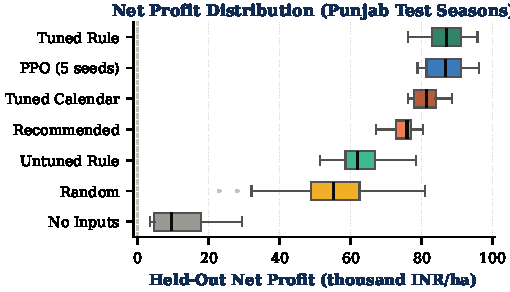
\includegraphics[width=0.96\columnwidth,keepaspectratio]{profit_distribution}
    \caption{\textbf{Held-out Punjab net profit distributions (2017--2023):} PPO earns $+11{,}935\text{ INR/ha}$ (+16.0\%) over the recommended calendar and achieves $96.6\%$ of the hindsight oracle ceiling across 5 random seeds.}
    \label{fig:profit_dist}
\end{figure}

% =========================================================================
% PAGE 2: EXPERIMENTAL PROGRESSION, BEST MODEL & LESSONS LEARNED
% =========================================================================
\newpage
\section{Experimental Progression, Best Model, and Lessons Learned}
Table~\ref{tab:results} summarizes held-out benchmarking of all policies. Figure~\ref{fig:profit_dist} illustrates held-out profit distributions, while Figure~\ref{fig:sweeps} and Table~\ref{tab:ablations} detail the 12 systematic ablation studies across 5 seeds:

\textbf{1. Baseline Gap and Shapley Split:} Base PPO ($2\times64$ MLP, GAE $\lambda=0.95$, clip $\epsilon=0.2$) earns $86{,}584 \pm 153\text{ INR/ha}$, beating recommended extension advice by $+11{,}935\text{ INR/ha}$ (+16.0\%) and saving 26.7\% irrigation water (220 vs 300 mm). Shapley decomposition across all 24 decision coalitions reveals that 62\% of this gain arises from adaptive water timing and 31\% from nitrogen splits. PPO trails the tuned rule by $-648\text{ INR/ha}$ due to rainfall stochasticity.

\textbf{2. Optimization Invariance:} Sweeping learning rate decay, observation normalization, orthogonal initialization, reward discount $\gamma=1.0$, and extending training to 1M steps shifted profit by $<0.1\%$, proving that the gap was informational rather than algorithmic. Branching DQN ($83{,}617$) and CEM ($84{,}178$) lagged behind.

\textbf{3. Action Discretization:} Introducing a 4-level irrigation grid $\{0, 25, 50, 75\}\text{ mm}$ paired with a joint $N\times W$ action head lifted PPO to $86{,}821 \pm 315\text{ INR/ha}$, outperforming its own retuned rule across all seeds.

\textbf{4. Pest Severity Response:} Under severe pest loss ($L_p \ge 0.30$), PPO decisively outperforms the retuned rule across all seeds by $+2{,}601$ to $+3{,}827\text{ INR/ha}$ through resistance-aware selective spraying (3.59 vs 6.32 doses at $L_p=0.35$), preventing chemical resistance buildup.

\begin{figure}[t]
    \centering
    {\footnotesize\textbf{\color{primary}(a) Pest Severity Sweep ($L_p \in [0.115, 0.50]$)}}\\[0.5pt]
    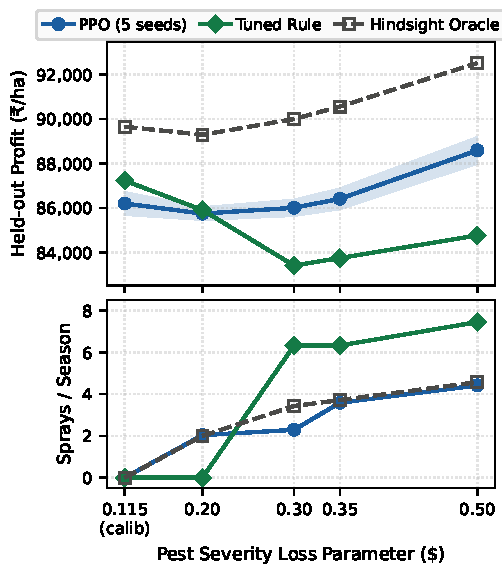
\includegraphics[width=0.54\columnwidth,keepaspectratio]{pest_sweep_pub}\\[1.5pt]
    {\footnotesize\textbf{\color{primary}(b) Action Layout \& Next-Fortnight Rain Forecast}}\\[0.5pt]
    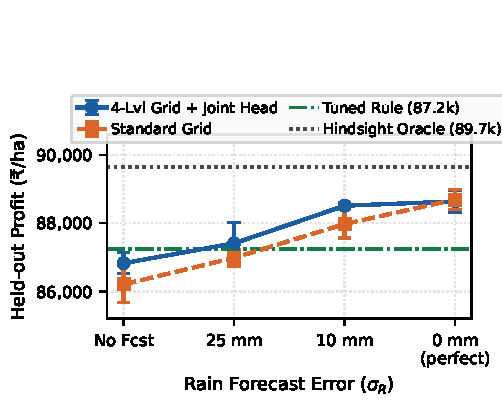
\includegraphics[width=0.58\columnwidth,keepaspectratio]{layout_forecast_pub}
    \caption{\textbf{Performance sweeps with zero-overlap legends:} \textbf{(a)} For pest loss $L_p \ge 0.30$, PPO beats the retuned rule across all seeds ($+2.6\text{k}$ to $+3.8\text{k INR/ha}$) via resistance-aware selective spraying. \textbf{(b)} Combining a 4-level water grid, joint head, and a $10\text{ mm}$ rain forecast achieves $88{,}508\pm 81\text{ INR/ha}$ ($98.9\%$ of oracle).}
    \label{fig:sweeps}
\end{figure}

\textbf{5. Best Model Discovery (Weather Foresight):} Oracle decomposition indicates that future weather clairvoyance is worth $+5{,}367\text{ INR/ha}$ vs $+188\text{ INR/ha}$ for price knowledge. Supplying a noisy 14-day rainfall forecast with error $\sigma_R = 10\text{ mm}$ to the 4-level joint agent produced our \textbf{best overall model: $88{,}508 \pm 81\text{ INR/ha}$} (\textbf{98.9\% of oracle ceiling}), beating the tuned rule by $+1{,}963\text{ INR/ha}$ across all 5 seeds.

\textbf{6. Critic-Free GRPO and Cross-State Transfer:} Critic-free GRPO matched PPO ($86{,}223$ vs $86{,}584\text{ INR/ha}$) with 6\% faster runtime. Zero-shot transfer from Punjab to Haryana achieved $74{,}303 \pm 463\text{ INR/ha}$ (96.2\% of Haryana oracle), exceeding Haryana's local tuned rule ($73{,}831\text{ INR/ha}$) without retraining.

\begin{center}
\vspace{1.0pt}
\captionof{table}{Systematic ablation and experiment breakdown across 5 seeds: progression from base PPO to the best foresight model.}
\label{tab:ablations}
\resizebox{\columnwidth}{!}{%
\setlength{\tabcolsep}{2.5pt}
\renewcommand{\arraystretch}{0.93}
\begin{tabular}{llrrrr}
\toprule
\rowcolor{tableheader}
\textbf{Study / Ablation} & \textbf{Intervention / Mechanism} & \textbf{Profit (INR/ha)} & \textbf{Gap to Rule} & \textbf{\% Orac.} & \textbf{Win} \\
\midrule
01: Base PPO & 3-lvl grid, separate heads & $86{,}584 \pm 153$ & $-648$ & $96.6\%$ & 0/5 \\
03: Action Layout & 4-lvl water + joint $N\times W$ & $86{,}821 \pm 315$ & $+621$ & $96.9\%$ & 5/5 \\
05: Severe Pest Loss & $L_p = 0.35$ (selective spray) & $86{,}410 \pm 492$ & $+2{,}664$ & $95.4\%$ & 5/5 \\
07: Weather Forecast & Standard grid, $\sigma_R = 10\text{ mm}$ & $87{,}972 \pm 412$ & $+586$ & $98.3\%$ & 4/5 \\
\rowcolor{cardbg}
\textbf{12: Best Model} & \textbf{4-lvl grid + $\sigma_R = 10\text{ mm}$ fcst} & $\mathbf{88{,}508 \pm 81}$ & $\mathbf{+1{,}963}$ & $\mathbf{98.9\%}$ & \textbf{5/5} \\
12: Perfect Weather & 4-lvl grid + clairvoyant rain & $88{,}635 \pm 317$ & $+1{,}403$ & $99.1\%$ & 5/5 \\
Transfer: Haryana & Zero-shot to Karnal climate & $74{,}303 \pm 463$ & $+472$ & $96.2\%$ & 5/5 \\
\bottomrule
\end{tabular}%
}
\vspace{1.0pt}
\end{center}

% =========================================================================
% SECTION 5: CONCLUSION & REFERENCES
% =========================================================================
\section{Conclusion}
FarmRL demonstrates that RL policies discover water-conserving, resistance-mitigating input schedules in complex agro-ecosystems. While tuned static heuristics suffice under predictable conditions, RL policies convincingly outperform them when pest damage is non-trivial and when conditioning on short-term rainfall forecasts. The project includes an interactive 7-page Streamlit decision dashboard.

\vspace{2.0pt}
\noindent{\footnotesize\textbf{\color{primary}References}}\\[1.0pt]
{\scriptsize
[1] CACP, \textit{Price Policy for Rabi Crops: RMS 2027--28 (Annex 5.6a)}, Govt. of India, 2026. \quad
[2] ICRISAT, TCI Cornell, \& IFPRI, \textit{District-Level Database for Indian Agriculture (1966--2017)}. \quad
[3] J.~Doorenbos \& A.~Kassam, \textit{Yield Response to Water}, FAO Paper 33, 1979; P.~Steduto et al., \textit{AquaCrop}, FAO Paper 66, 2012. \quad
[4] M.~Rodell et al., ``Satellite groundwater depletion in India,'' \textit{Nature}, 460:999--1002, 2009. \quad
[5] J.~Schulman et al., ``PPO Algorithms,'' \textit{arXiv:1707.06347}, 2017; Z.~Shao et al., ``DeepSeekMath (GRPO),'' \textit{arXiv:2402.03300}, 2024.\par
}

\end{document}
